% Generated by fikzPy
\documentclass[tikz,border=0pt]{standalone}
\usepackage{tikz}

\begin{document}
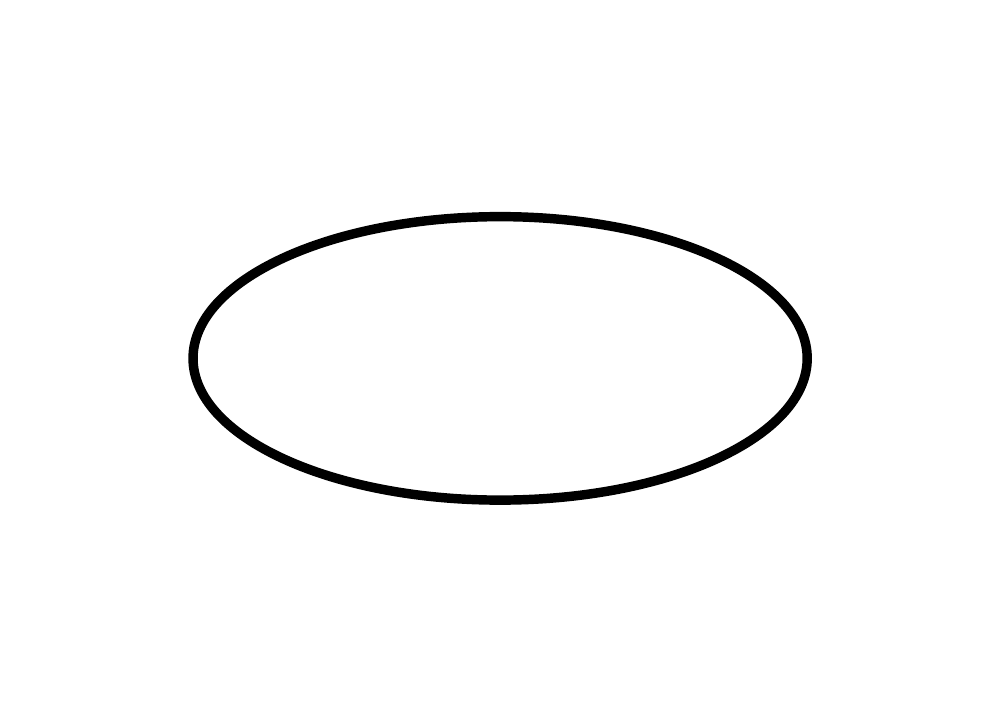
\begin{tikzpicture}[scale=1]
  \begin{scope}
  \clip (0,0) rectangle (12.0,8.4);

  \draw[draw=none,draw=black,line width=0.12cm] (9.9, 4.2).. controls (9.9, 3.7029) and (9.4635, 3.2529) .. (8.7577, 2.9272).. controls (8.052, 2.6015) and (7.077, 2.4) .. (6.0, 2.4).. controls (4.923, 2.4) and (3.948, 2.6015) .. (3.2423, 2.9272).. controls (2.5365, 3.2529) and (2.1, 3.7029) .. (2.1, 4.2).. controls (2.1, 4.6971) and (2.5365, 5.1471) .. (3.2423, 5.4728).. controls (3.948, 5.7985) and (4.923, 6.0) .. (6.0, 6.0).. controls (7.077, 6.0) and (8.052, 5.7985) .. (8.7577, 5.4728).. controls (9.4635, 5.1471) and (9.9, 4.6971) .. (9.9, 4.2) -- cycle;




\end{scope}
\pgfresetboundingbox
\path[use as bounding box] (0,0) rectangle (12.0,8.4);
\end{tikzpicture}
\end{document}
